


    Apêndice 1 - Resultado do Circuito \textit{Biquad Highpass Filter}
    
    
        \begin{figure}[H]
        \begin{center}
        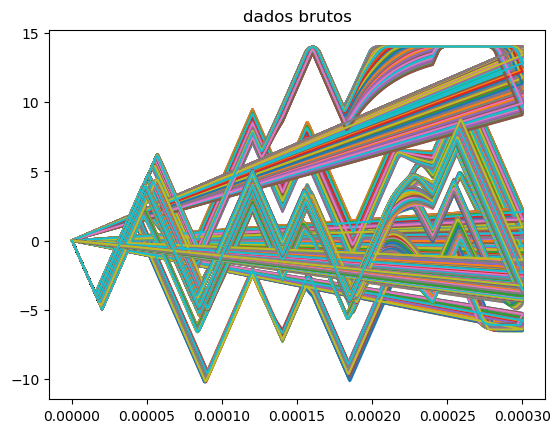
\includegraphics[width=13cm]{./01_Pre_textuais/biquad_figs/brutos_BiquadHighpassFiltermc+4bitPRBS[FALHA]raw.png}
        \caption{\label{fig:dadoBrutoPAA}- Circuito: Biquad - Dados recém adquiridos.}
        \end{center}
        \end{figure}
        
        \begin{figure}[H]
        \begin{center}
        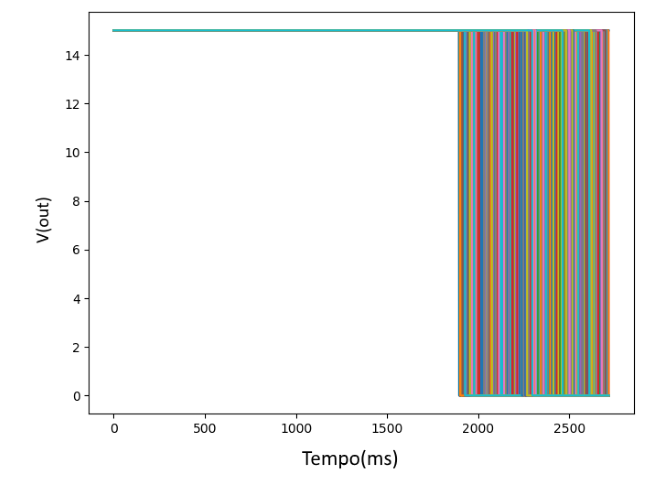
\includegraphics[width=13cm]{./01_Pre_textuais/biquad_figs/dadosPreProc_Biquad_Highpass_Filter_mc_+_4bitPRBS_[FALHA]raw.png}
        \caption{\label{fig:dadoPAA}- Circuito: Biquad - Dados após passarem por pré-processamento.}
        \end{center}
        \end{figure}
        
        \begin{figure}[H]
        \begin{center}
        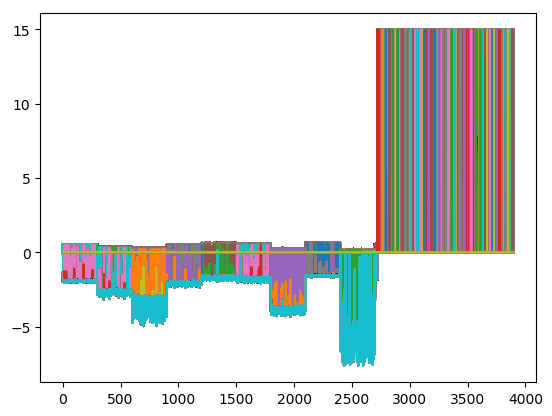
\includegraphics[width=13cm]{./01_Pre_textuais/biquad_figs/PAA_Biquad_Highpass_Filter_mc_+_4bitPRBS_[FALHA]raw.png}
        \caption{\label{fig:paaSalenkey}- Circuito: Biquad -Todas Dados antes da aplicação do PCA}
        \end{center}
        \end{figure}
        
        
        \begin{figure}[H]
        \begin{center}
        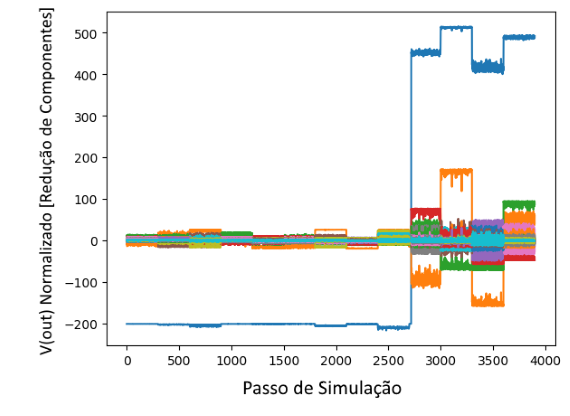
\includegraphics[width=13cm]{./01_Pre_textuais/biquad_figs/PCA_Biquad_Highpass_Filter_mc_+_4bitPRBS_[FALHA]raw.png}
        \caption{\label{fig:pcaSalenkey}- Circuito: Biquad -Todas Dados depois da aplicação do PCA}
        \end{center}
        \end{figure}
        
        \begin{figure}[H]
        \begin{center}
        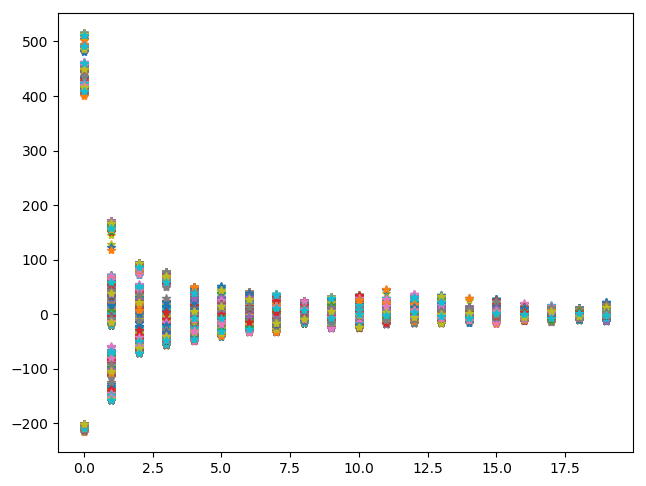
\includegraphics[width=13cm]{./01_Pre_textuais/biquad_figs/dadosPosPCA_Biquad_Highpass_Filter_mc_+_4bitPRBS_[FALHA]raw.png}
        \caption{\label{fig:pcaAPOSSalenkey}- Circuito: Biquad - Variância por componente do PCA}
        \end{center}
        \end{figure}
        
        \begin{figure}[H]
        \begin{center}
        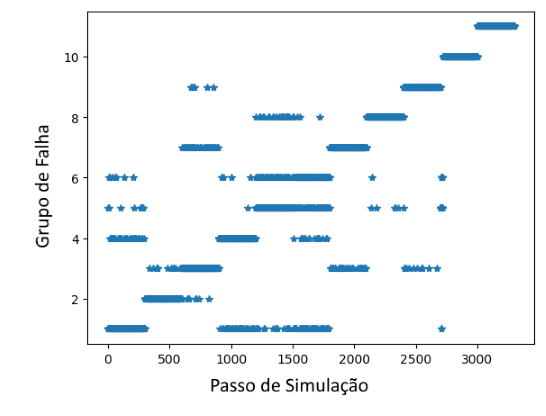
\includegraphics[width=13cm]{./01_Pre_textuais/biquad_figs/AdaBoostClassifier_Biquad_Highpass_Filter_mc_+_4bitPRBS_[FALHA]raw.png}
        \caption{\label{fig:DecisionTreeClassifieSalenkey}- Circuito: Biquad - Comportamento da Predição Ada Boost}
        \end{center}
        \end{figure}
       
       
        \begin{figure}[H]
        \begin{center}
        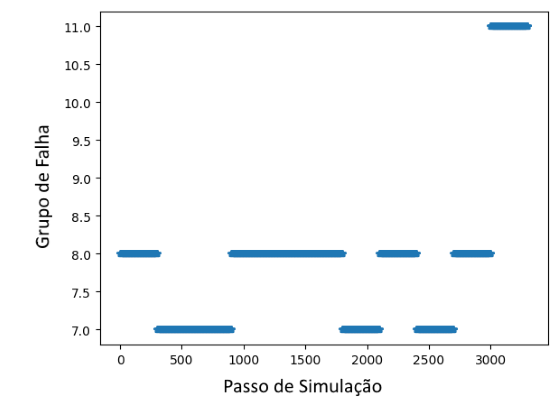
\includegraphics[width=13cm]{./01_Pre_textuais/biquad_figs/SVC_Biquad_Highpass_Filter_mc_+_4bitPRBS_[FALHA]raw.png}
        \caption{\label{fig:DecisionTreeClassifieSalenkey}- Circuito: Biquad - Comportamento da Predição SVC}
        \end{center}
        \end{figure}
        
        \begin{figure}[H]
        \begin{center}
        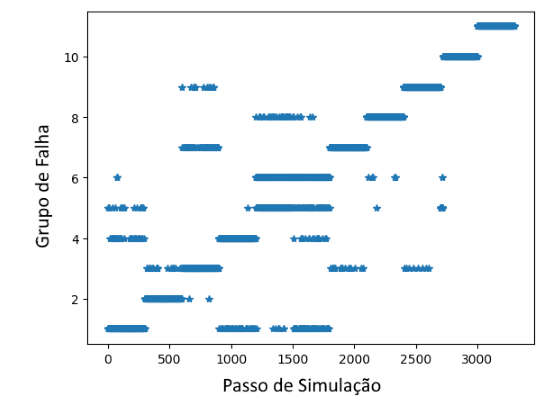
\includegraphics[width=13cm]{./01_Pre_textuais/biquad_figs/RandomForestClassifier_Biquad_Highpass_Filter_mc_+_4bitPRBS_[FALHA]raw.png}
        \caption{\label{fig:DecisionTreeClassifieSalenkey}- Circuito: Biquad - Comportamento da Predição Random Forest }
        \end{center}
        \end{figure}
        
        \begin{figure}[H]
        \begin{center}
        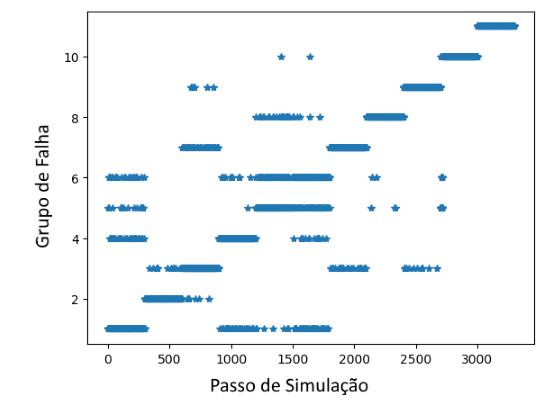
\includegraphics[width=13cm]{./01_Pre_textuais/biquad_figs/GaussianNB_Biquad_Highpass_Filter_mc_+_4bitPRBS_[FALHA]raw.png}
        \caption{\label{fig:DecisionTreeClassifieSalenkey}- Circuito: Biquad - Comportamento Predição GaussianNB}
        \end{center}
        \end{figure}
        
        
        \begin{figure}[H]
        \begin{center}
        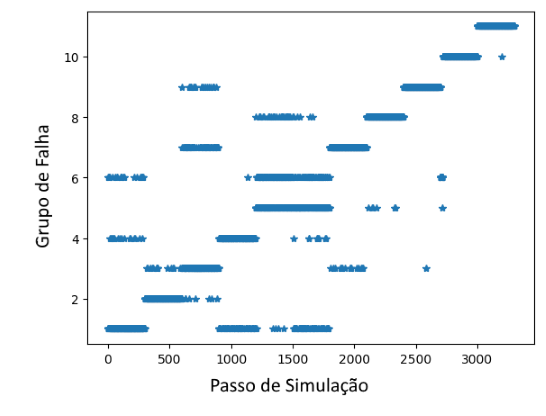
\includegraphics[width=13cm]{./01_Pre_textuais/biquad_figs/KNeighborsClassifier_Biquad_Highpass_Filter_mc_+_4bitPRBS_[FALHA]raw.png}
        \caption{\label{fig:DecisionTreeClassifieSalenkey}- Circuito: Biquad - Comportamento da Predição K-Neighbors }
        \end{center}
        \end{figure}
        
        
        \begin{figure}[H]
        \begin{center}
        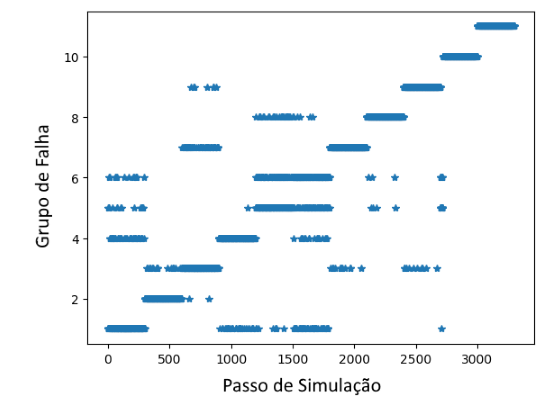
\includegraphics[width=13cm]{./01_Pre_textuais/biquad_figs/SGDClassifier_Biquad_Highpass_Filter_mc_+_4bitPRBS_[FALHA]raw.png}
        \caption{\label{fig:DecisionTreeClassifieSalenkey}- Circuito: Biquad - Comportamento da Predição SGD}
        \end{center}
        \end{figure}
        
        
        \begin{figure}[H]
        \begin{center}
        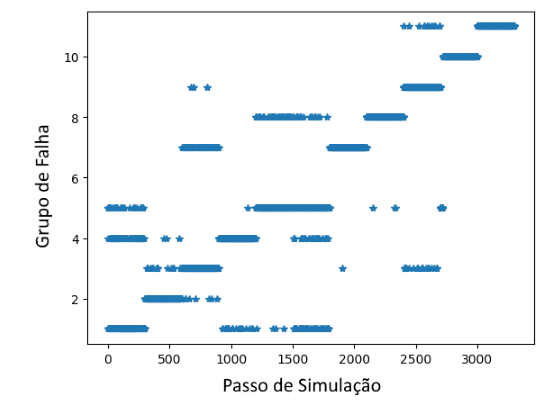
\includegraphics[width=13cm]{./01_Pre_textuais/biquad_figs/LogisticRegression_Biquad_Highpass_Filter_mc_+_4bitPRBS_[FALHA]raw.png}
        \caption{\label{fig:DecisionTreeClassifieSalenkey}- Circuito: Biquad - Comportamento da Predição Logistic Regression }
        \end{center}
        \end{figure}
        
       
        
        \begin{figure}[H]
        \begin{center}
        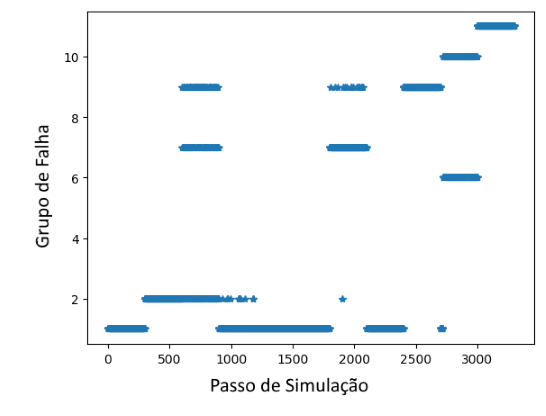
\includegraphics[width=13cm]{./01_Pre_textuais/biquad_figs/KMeans_Biquad_Highpass_Filter_mc_+_4bitPRBS_[FALHA]raw.png}
        \caption{\label{fig:DecisionTreeClassifieSalenkey}- Circuito: Biquad - Comportamento da Predição KMeans }
        \end{center}
        \end{figure}
        
        \begin{figure}[H]
        \begin{center}
        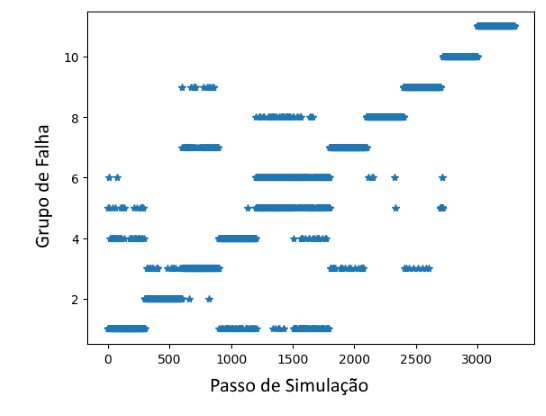
\includegraphics[width=13cm]{./01_Pre_textuais/biquad_figs/GMM_Biquad_Highpass_Filter_mc_+_4bitPRBS_[FALHA]raw.png}
        \caption{\label{fig:DecisionTreeClassifieSalenkey}- Circuito: Biquad - Comportamento da Predição GMM }
        \end{center}
        \end{figure}
        

    
    %saidas dos treinamentos igual pagina 40 -41 GSC
    
    
    \newpage
    Apêndice 2 - Resultado do Circuito CTSV
    
    \begin{figure}[H]
        \begin{center}
        \includegraphics[width=13cm]{./01_Pre_textuais/ctsv_figs/brutos_CTSV4bitPRBS[FALHA]raw.png}
        \caption{\label{fig:dadoBrutoPAA}- Circuito: CTSV - Dados recém adquiridos.}
        \end{center}
        \end{figure}
        
        \begin{figure}[H]
        \begin{center}
        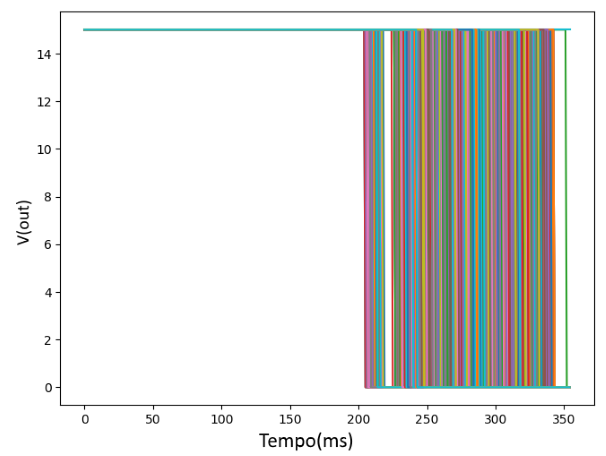
\includegraphics[width=13cm]{./01_Pre_textuais/ctsv_figs/dadosPreProc_CTSV_mc_+_4bitPRBS_[FALHA]raw.png}
        \caption{\label{fig:dadoPAA}- Circuito:CTSV - Dados após passarem por pré-processamento.}
        \end{center}
        \end{figure}
        
        \begin{figure}[H]
        \begin{center}
        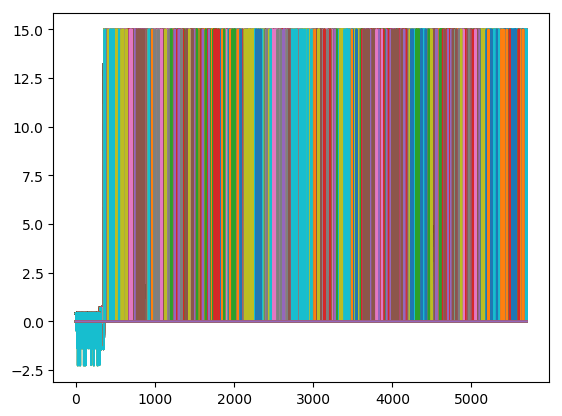
\includegraphics[width=13cm]{./01_Pre_textuais/ctsv_figs/PAA_CTSV_mc_+_4bitPRBS_[FALHA]raw.png}
        \caption{\label{fig:paaSalenkey}- Circuito: CTSV -Todas Dados antes da aplicação do PCA}
        \end{center}
        \end{figure}
        
        
        \begin{figure}[H]
        \begin{center}
        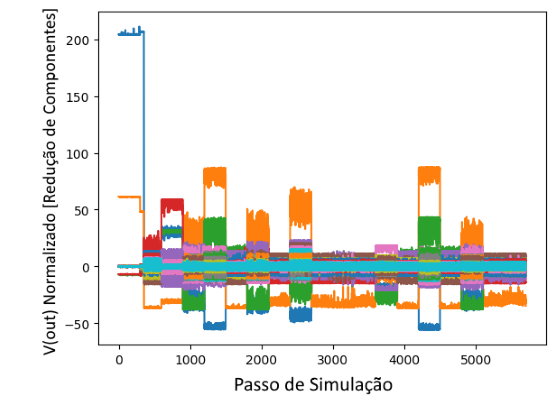
\includegraphics[width=13cm]{./01_Pre_textuais/ctsv_figs/PCA_CTSV_mc_+_4bitPRBS_[FALHA]raw.png}
        \caption{\label{fig:pcaSalenkey}- Circuito: CTSV  -Todas Dados depois da aplicação do PCA}
        \end{center}
        \end{figure}
        
        \begin{figure}[H]
        \begin{center}
        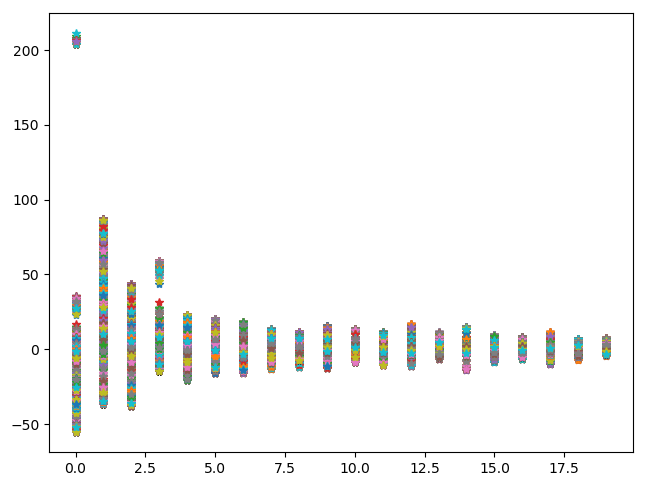
\includegraphics[width=13cm]{./01_Pre_textuais/ctsv_figs/dadosPosPCA_CTSV_mc_+_4bitPRBS_[FALHA]raw.png}
        \caption{\label{fig:pcaAPOSSalenkey}- Circuito: CTSV - Variância por componente do PCA}
        \end{center}
        \end{figure}
        
        \begin{figure}[H]
        \begin{center}
        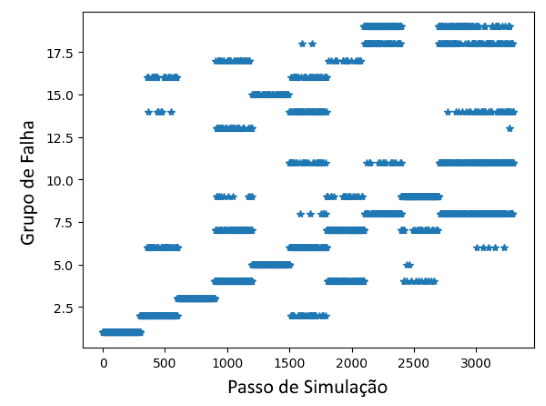
\includegraphics[width=13cm]{./01_Pre_textuais/ctsv_figs/AdaBoostClassifier_CTSV_mc_+_4bitPRBS_[FALHA]raw.png}
        \caption{\label{fig:DecisionTreeClassifieSalenkey}- Circuito: CTSV - Comportamento da Predição Ada Boost}
        \end{center}
        \end{figure}
       
       
        \begin{figure}[H]
        \begin{center}
        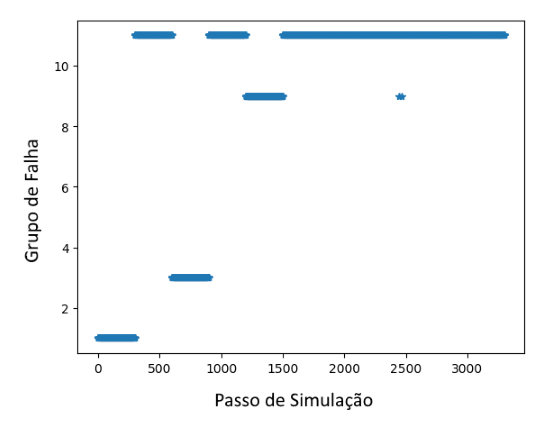
\includegraphics[width=13cm]{./01_Pre_textuais/ctsv_figs/SVC_CTSV_mc_+_4bitPRBS_[FALHA]raw.png}
        \caption{\label{fig:DecisionTreeClassifieSalenkey}- Circuito: CTSV - Comportamento da Predição SVC}
        \end{center}
        \end{figure}
        
        \begin{figure}[H]
        \begin{center}
        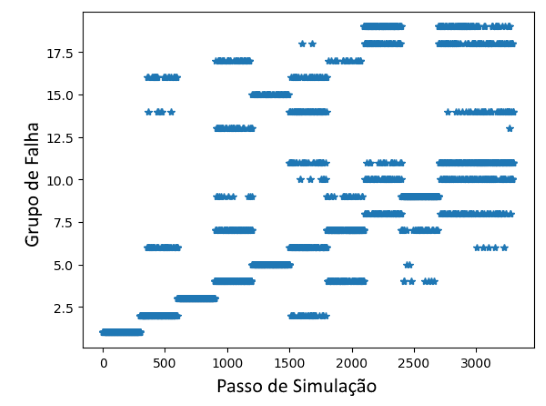
\includegraphics[width=13cm]{./01_Pre_textuais/ctsv_figs/RandomForestClassifier_CTSV_mc_+_4bitPRBS_[FALHA]raw.png}
        \caption{\label{fig:DecisionTreeClassifieSalenkey}- Circuito: CTSV - Comportamento da Predição Random Forest }
        \end{center}
        \end{figure}
        
        \begin{figure}[H]
        \begin{center}
        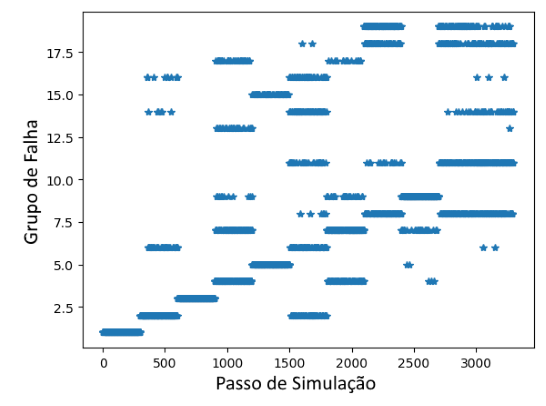
\includegraphics[width=13cm]{./01_Pre_textuais/ctsv_figs/GaussianNB_CTSV_mc_+_4bitPRBS_[FALHA]raw.png}
        \caption{\label{fig:DecisionTreeClassifieSalenkey}- Circuito: CTSV - Comportamento Predição GaussianNB}
        \end{center}
        \end{figure}
        
        
        \begin{figure}[H]
        \begin{center}
        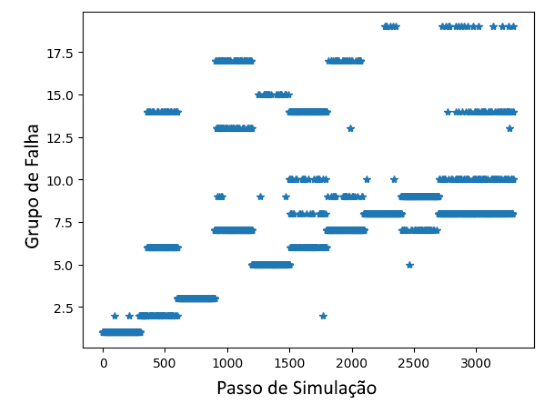
\includegraphics[width=13cm]{./01_Pre_textuais/ctsv_figs/KNeighborsClassifier_CTSV_mc_+_4bitPRBS_[FALHA]raw.png}
        \caption{\label{fig:DecisionTreeClassifieSalenkey}- Circuito: CTSV - Comportamento da Predição K-Neighbors }
        \end{center}
        \end{figure}
        
        
        \begin{figure}[H]
        \begin{center}
        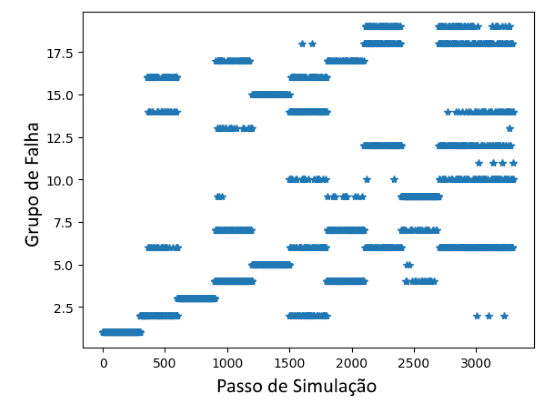
\includegraphics[width=13cm]{./01_Pre_textuais/ctsv_figs/SGDClassifier_CTSV_mc_+_4bitPRBS_[FALHA]raw.png}
        \caption{\label{fig:DecisionTreeClassifieSalenkey}- Circuito: CTSV - Comportamento da Predição SGD}
        \end{center}
        \end{figure}
        
        
        \begin{figure}[H]
        \begin{center}
        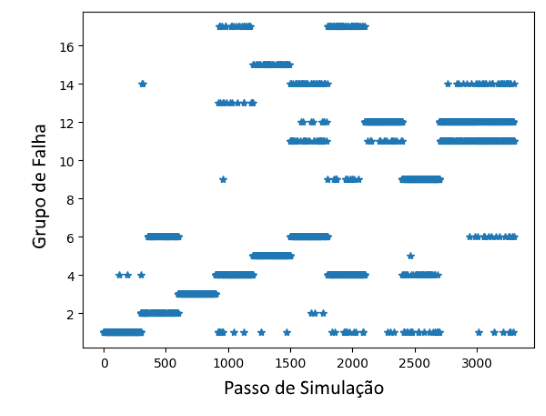
\includegraphics[width=13cm]{./01_Pre_textuais/ctsv_figs/LogisticRegression_CTSV_mc_+_4bitPRBS_[FALHA]raw.png}
        \caption{\label{fig:DecisionTreeClassifieSalenkey}- Circuito: CTSV - Comportamento da Predição Logistic Regression }
        \end{center}
        \end{figure}
        
       
        
        \begin{figure}[H]
        \begin{center}
        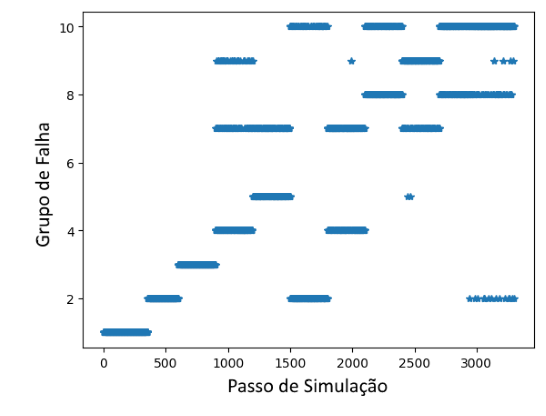
\includegraphics[width=13cm]{./01_Pre_textuais/ctsv_figs/KMeans_CTSV_mc_+_4bitPRBS_[FALHA]raw.png}
        \caption{\label{fig:DecisionTreeClassifieSalenkey}- Circuito: CTSV - Comportamento da Predição KMeans }
        \end{center}
        \end{figure}
        
        \begin{figure}[H]
        \begin{center}
        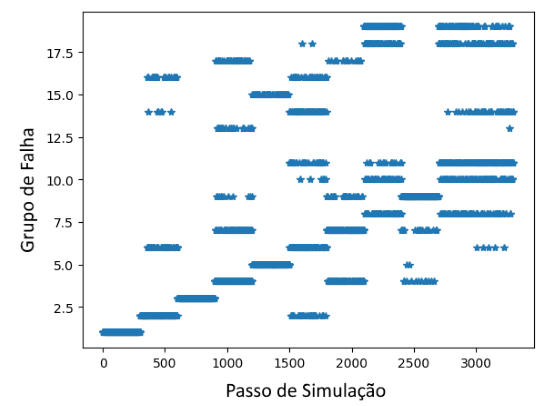
\includegraphics[width=13cm]{./01_Pre_textuais/ctsv_figs/GMM_CTSV_mc_+_4bitPRBS_[FALHA]raw.png}
        \caption{\label{fig:DecisionTreeClassifieSalenkey}- Circuito: CTSV - Comportamento da Predição GMM }
        \end{center}
        \end{figure}
    
    
     %saidas dos treinamentos igual pagina 40 -41 GSC
    
    
    
    
    \newpage
    Apêndice 3 - Resultado do Circuito Nonlinear Rectfier
    
    
    
      \begin{figure}[H]
        \begin{center}
        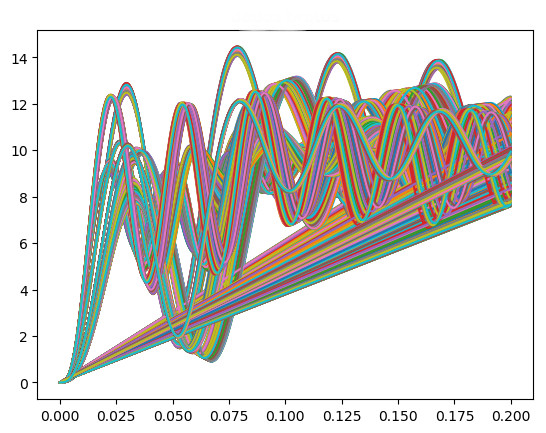
\includegraphics[width=13cm]{./01_Pre_textuais/nonlin_figs/brutosNon.png}
        \caption{\label{fig:dadoBrutoPAA}- Circuito: Nonlinear Rectifier - Dados recém adquiridos.}
        \end{center}
        \end{figure}
        
        \begin{figure}[H]
        \begin{center}
        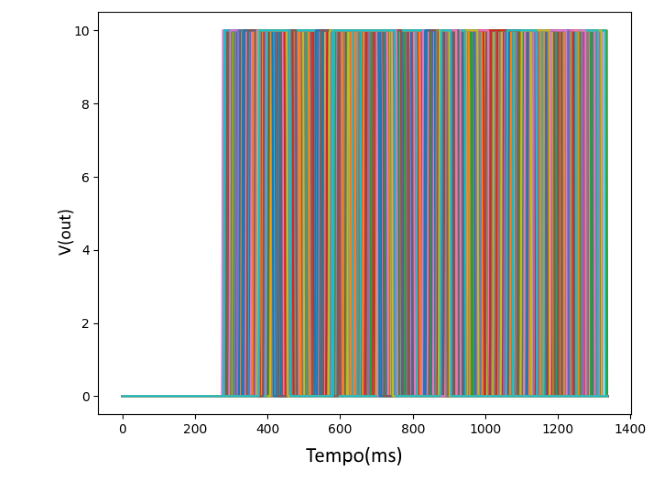
\includegraphics[width=13cm]{./01_Pre_textuais/nonlin_figs/dadosPreProc_Nonlinear_Rectfier_+_4bit_PRBS_[FALHA]_-_300_-_02sraw.png}
        \caption{\label{fig:dadoPAA}- Circuito:CTSV - Dados após passarem por pré-processamento.}
        \end{center}
        \end{figure}
        
        \begin{figure}[H]
        \begin{center}
        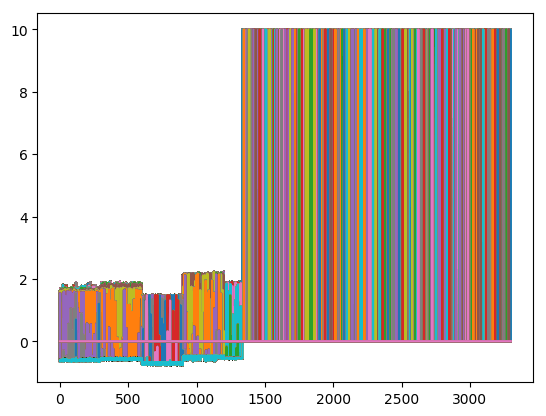
\includegraphics[width=13cm]{./01_Pre_textuais/nonlin_figs/PAA_Nonlinear_Rectfier_+_4bit_PRBS_[FALHA]_-_300_-_02sraw.png}
        \caption{\label{fig:paaSalenkey}- Circuito: Nonlinear Rectifier -Todas Dados antes da aplicação do PCA}
        \end{center}
        \end{figure}
        
        
        \begin{figure}[H]
        \begin{center}
        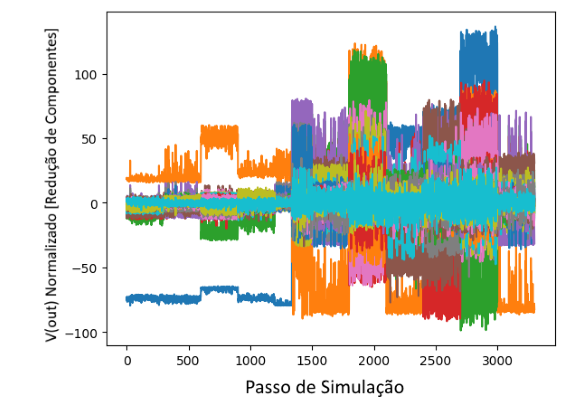
\includegraphics[width=13cm]{./01_Pre_textuais/nonlin_figs/PCA_Nonlinear_Rectfier_+_4bit_PRBS_[FALHA]_-_300_-_02sraw.png}
        \caption{\label{fig:pcaSalenkey}- Circuito: Nonlinear Rectifier  -Todas Dados depois da aplicação do PCA}
        \end{center}
        \end{figure}
        
        \begin{figure}[H]
        \begin{center}
        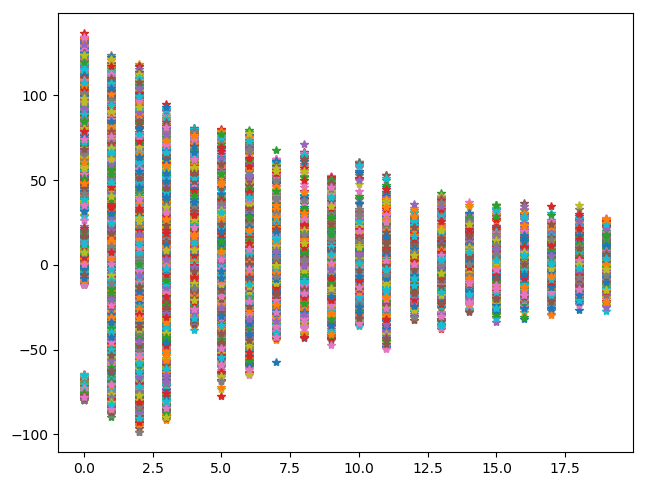
\includegraphics[width=13cm]{./01_Pre_textuais/nonlin_figs/dadosPosPCA_Nonlinear_Rectfier_+_4bit_PRBS_[FALHA]_-_300_-_02sraw.png}
        \caption{\label{fig:pcaAPOSSalenkey}- Circuito: Nonlinear Rectifier - Variância por componente do PCA}
        \end{center}
        \end{figure}
        
        \begin{figure}[H]
        \begin{center}
        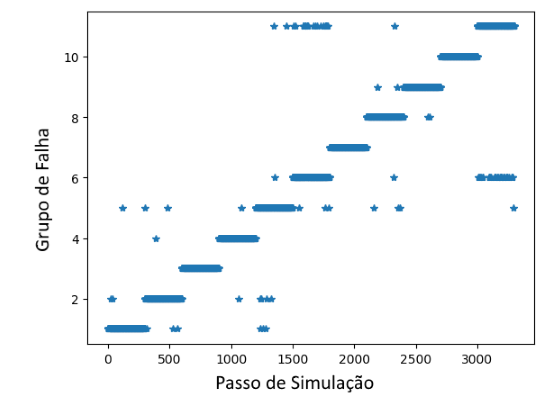
\includegraphics[width=13cm]{./01_Pre_textuais/nonlin_figs/AdaBoostClassifier_Nonlinear_Rectfier_+_4bit_PRBS_[FALHA]_-_300_-_02sraw.png}
        \caption{\label{fig:DecisionTreeClassifieSalenkey}- Circuito: Nonlinear Rectifier - Comportamento da Predição Ada Boost}
        \end{center}
        \end{figure}
       
       
        \begin{figure}[H]
        \begin{center}
        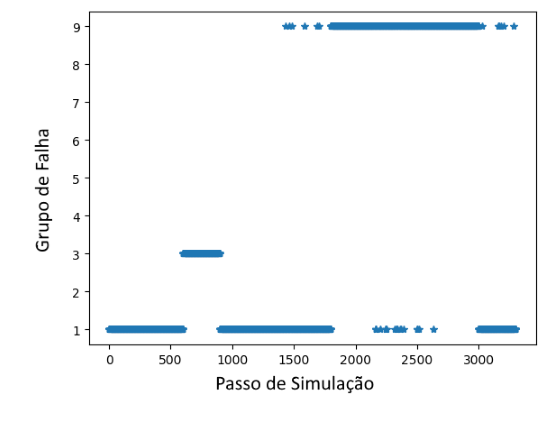
\includegraphics[width=13cm]{./01_Pre_textuais/nonlin_figs/SVC_Nonlinear_Rectfier_+_4bit_PRBS_[FALHA]_-_300_-_02sraw.png}
        \caption{\label{fig:DecisionTreeClassifieSalenkey}- Circuito: Nonlinear Rectifier - Comportamento da Predição SVC}
        \end{center}
        \end{figure}
        
        \begin{figure}[H]
        \begin{center}
        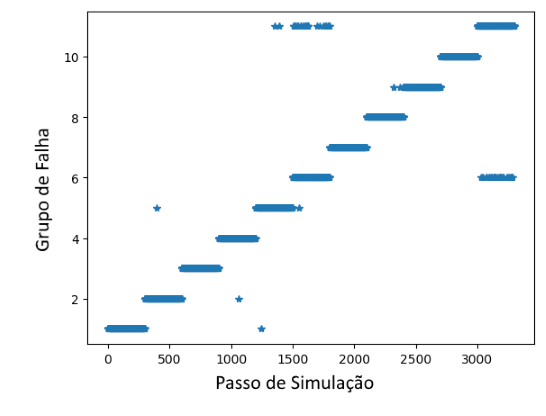
\includegraphics[width=13cm]{./01_Pre_textuais/nonlin_figs/RandomForestClassifier_Nonlinear_Rectfier_+_4bit_PRBS_[FALHA]_-_300_-_02sraw.png}
        \caption{\label{fig:DecisionTreeClassifieSalenkey}- Circuito: Nonlinear Rectifier - Comportamento da Predição Random Forest }
        \end{center}
        \end{figure}
        
        \begin{figure}[H]
        \begin{center}
        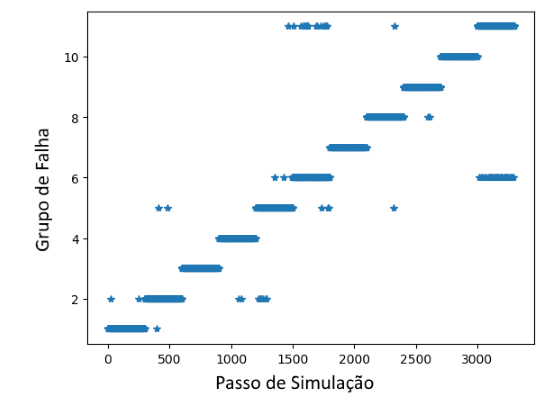
\includegraphics[width=13cm]{./01_Pre_textuais/nonlin_figs/GaussianNB_Nonlinear_Rectfier_+_4bit_PRBS_[FALHA]_-_300_-_02sraw.png}
        \caption{\label{fig:DecisionTreeClassifieSalenkey}- Circuito: Nonlinear Rectifier - Comportamento Predição GaussianNB}
        \end{center}
        \end{figure}
        
        
        \begin{figure}[H]
        \begin{center}
        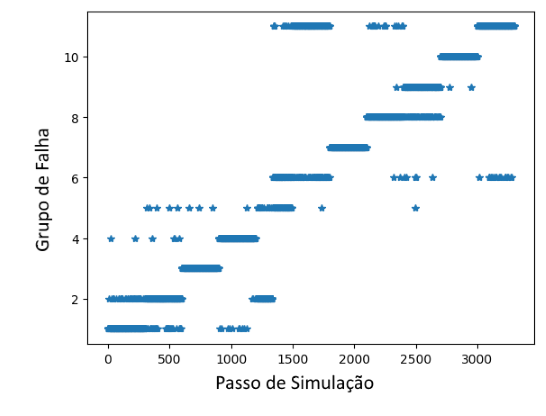
\includegraphics[width=13cm]{./01_Pre_textuais/nonlin_figs/KNeighborsClassifier_Nonlinear_Rectfier_+_4bit_PRBS_[FALHA]_-_300_-_02sraw.png}
        \caption{\label{fig:DecisionTreeClassifieSalenkey}- Circuito: Nonlinear Rectifier - Comportamento da Predição K-Neighbors }
        \end{center}
        \end{figure}
        
        
        \begin{figure}[H]
        \begin{center}
        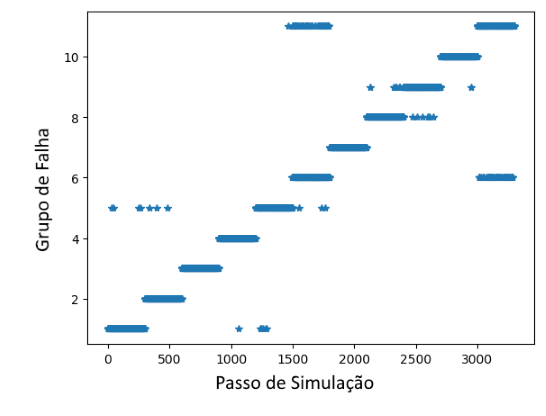
\includegraphics[width=13cm]{./01_Pre_textuais/nonlin_figs/SGDClassifier_Nonlinear_Rectfier_+_4bit_PRBS_[FALHA]_-_300_-_02sraw.png}
        \caption{\label{fig:DecisionTreeClassifieSalenkey}- Circuito: Nonlinear Rectifier - Comportamento da Predição SGD}
        \end{center}
        \end{figure}
        
        
        \begin{figure}[H]
        \begin{center}
        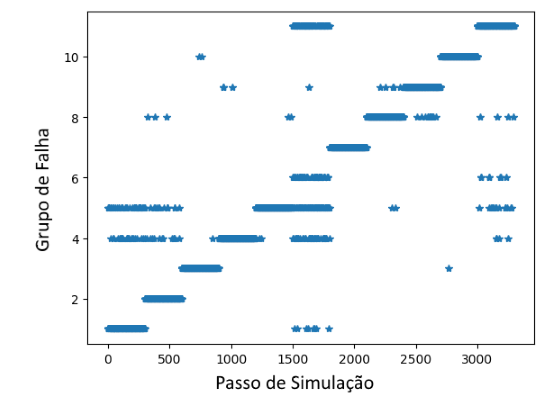
\includegraphics[width=13cm]{./01_Pre_textuais/nonlin_figs/LogisticRegression_Nonlinear_Rectfier_+_4bit_PRBS_[FALHA]_-_300_-_02sraw.png}
        \caption{\label{fig:DecisionTreeClassifieSalenkey}- Circuito: Nonlinear Rectifier - Comportamento da Predição Logistic Regression }
        \end{center}
        \end{figure}
        
       
        
        \begin{figure}[H]
        \begin{center}
        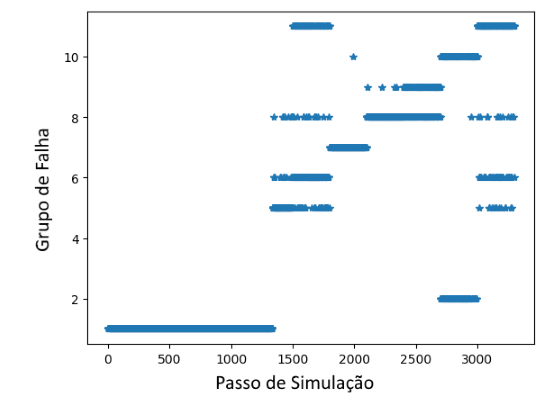
\includegraphics[width=13cm]{./01_Pre_textuais/nonlin_figs/KMeans_Nonlinear_Rectfier_+_4bit_PRBS_[FALHA]_-_300_-_02sraw.png}
        \caption{\label{fig:DecisionTreeClassifieSalenkey}- Circuito: Nonlinear Rectifier - Comportamento da Predição KMeans }
        \end{center}
        \end{figure}
        
        \begin{figure}[H]
        \begin{center}
        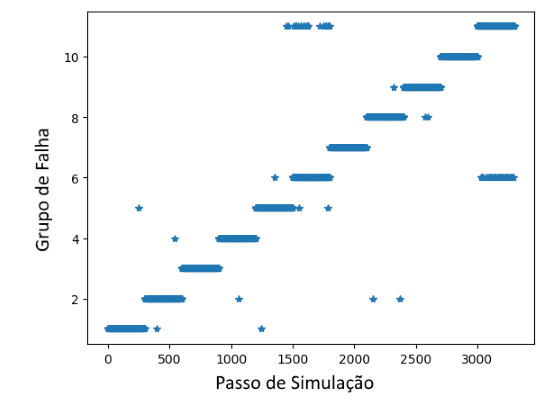
\includegraphics[width=13cm]{./01_Pre_textuais/nonlin_figs/GMM_Nonlinear_Rectfier_+_4bit_PRBS_[FALHA]_-_300_-_02sraw.png}
        \caption{\label{fig:DecisionTreeClassifieSalenkey}- Circuito: Nonlinear Rectifier - Comportamento da Predição GMM }
        \end{center}
        \end{figure}
    